\documentclass{llncs}
\usepackage[latin1]{inputenc}
%\usepackage[T1]{fontenc}
%\usepackage{textcomp}
%\usepackage{graphicx}
\usepackage{color}
%\usepackage{setspace}
\usepackage{url}
\usepackage[english]{babel}
\usepackage[pdftex]{graphicx}
\usepackage{epstopdf}
\usepackage{amsfonts}

\begin{document}

%
%     %%%%%%%%%%   TITLE   %%%%%%%%%%
%

% Tentative of (catchy) title
\title{Evil Evolves: Improving Generalized Flocking Strategies through Genetic Algorithm for the Ghost Team in the Game of Ms. Pac-Man}
% If the catchy title is a no-no, the following is suggested:
%\title{Improving Generalized Flocking Strategies through Genetic
%Algorithm: an Application to the Ms. Pac-Man vs Ghosts Competition}
% I like it, but better "Evolving Evil" o "Evolved Evil" Improving
% with respect to what? - JJ

%
%     %%%%%%%%%%   AUTHORS   %%%%%%%%%%
%
%\author{F. Liberatore, A.M. Mora}
%\authorrunning{F. Liberatore, A.M. Mora}
%\institute{
%Departamento de Arquitectura y Tecnología de Computadores. \\
%CITIC-UGR, ETSIIT. \\
%University of Granada, Spain \\
%\email{federico.liberatore@urjc.es, amorag@geneura.ugr.es}
%}

\maketitle

%
%     %%%%%%%%%%   ABSTRACT   %%%%%%%%%%
%
\begin{abstract} 
 Flocking Strategies % What are they?
allow to devise controllers with reduced
 computational complexity while generating emerging intelligent % emerging por qu�?
 behavior.  In this paper, we present an application of Genetic
 Algorithms and Flocking Strategies to control the Ghost Team in the
 game Ms. Pac-Man.The Ghost Team controllers are optimized for
 robustness by means of Genetic Algorithms  with respect to the
 stochastic elements of the game and effectivity against different
 possible opponents. The performance of the methodology proposed is
 tested and compared with that of other controllers. 
\end{abstract}
\textbf{Keywords.} Flocking, Genetic Algorithms, Artificial Intelligence, Ms. Pac-Man, Video Games, Evolutionary Computation.

%
%     %%%%%%%%%%   INTRODUCTION   %%%%%%%%%%
%
\section{Introduction}
\label{sec:intro}

Videogames such as Ms. Pac-Man are an ideal testbed for computational
intelligence as they allow for the confrontation of multiple
intelligent agents in a simple, yet challenging, context. The
Ms. Pac-Man vs Ghosts competition has been run since
2009. %reference - JJ
 Participants can submit controllers for either Ms. Pac-Man or
for the Ghost Team. % Which are the winners? How do they work? - JJ

In this work, an evolved controller for the Ghost Team based on
Genetic Programming and Flocking Strategies is proposed.  % Why? Will
                                % it be better than the state of the
                                % art? Do you want to compete? - JJ
                      
Flocking
Strategies consist of simple rules for the interactions of the
agents. Despite being computationally inexpensive, they often result
% lightweight?  You haven't described them yet. Flocking strategies
% are... - JJ
in complex emerging intelligent behaviors. We coupled Flocking
Strategies with Genetic Algorithms to design Ghost Team controllers
that are effective at minimizing Ms. Pac-Man final score and that are
also robust with respect to the stochastic elements of the game. 

% This should go to state of the art or as a justification of the work
% - JJ 
Although most of the research in this field focused on the design of
controllers for Ms. Pac-Man, a number of works regarding the Ghost
Team have been proposed. Nguyen and Ruck \cite{Nguyen2011,Nguyen2013}
present a controller based on Monte Carlo Tree Search where the
behavior of Ms. Pac-Man is simulated. Their controller won the first
Ms. Pac-Man Versus Ghost Team Competition held in 2011. Svensson and
Johansson \cite{Svensson2012} exploit the behavior emerging
capabilities of Influence Maps. A different line of research is
pursued by Sombat \textit{et al.} \cite{Sombat2012} that analyze
Ms. Pac-Man matches to classify Ghost Team controllers according to
their enjoyability and, therefore, understand the attribute that a
NPCs should posses for players to be engaged.

% you haven't said what is your objective in this paper, just doing a
% controller is not enough. Do you want to make it faster? Better?
% More robust? How will you measure/prove that? - JJ

The rest of the paper is organized as follows. The next section presents the Ms. Pac-Man problem description, including the competition features and restrictions. Some preliminary concepts and background of the work, along with related literature is commented in Section \ref{sec:preliminaryconcepts_sota}. Subsequently, Section \ref{sec:ghosts_ai} introduces the ghosts' AI approach which will be analyzed in the paper. Then the set of experiments conducted to perform this analysis is presented in Section \ref{sec:experiments}. Finally, Section \ref{sec:conclusions} describes the reached conclusions and outlines some future lines of work.

%
%     %%%%%%%%%%   PROBLEM DESCRIPTION   %%%%%%%%%%
%

\section{Ms Pac-Man. The Game and the Problem}
\label{sec:mspacman_problem}

The game of Pac-Man needs no presentation. Since its release in 1980 many variants have been proposed and Ms. Pac-Man was one of them. Released in 1981, Ms. Pac-Man presented several features that extended on the original game, such as a female character, new maze designs and several game-play changes. A screen-shot of the game is shown in Figure \ref{fig:mspacman_game_snap}.

\begin{figure}
\begin{center}
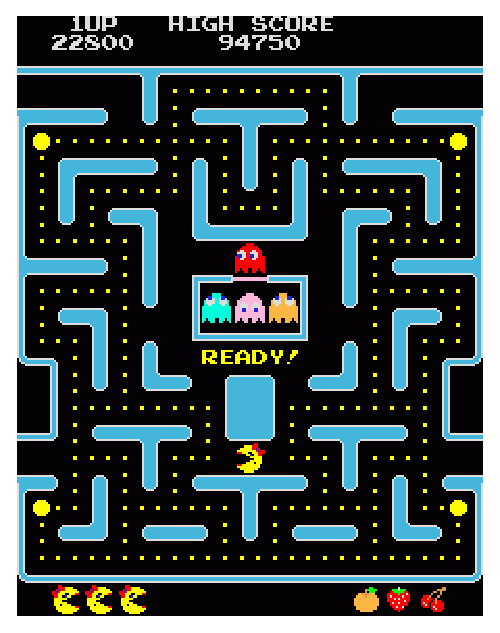
\includegraphics[scale=0.8]{img/mspacman.eps}
\caption{A screenshot from the Ms Pac-man game.
\label{fig:mspacman_game_snap}}
\end{center} % si no necesita presentaci�n, tampoco necesita este
             % gr�fico que hace que te pases de p�ginas - JJ
\end{figure}

In this game, Ms. Pac-Man has to collect all the pills in the maze
while avoiding the four ghosts chasing her. If Ms. Pac-Man is reached
by a ghost the player loses one life, Ms. Pac-Man is relocated at the
initial position, and the ghosts respawn from the center of the
maze. The {\em powerpills} located in the corners of the maze turn the ghosts edible for a short time, allowing Ms. Pac-Man to eat them. When a ghost gets eaten, it disappears from the game and respawns at the center of the maze after a certain amount of time. As the levels are cleared, the game becomes more difficult by changing certain parameters such as respawn time, length of time the ghosts are edible, and ghosts speed. Differently from the game of Pac-Man, this game has elements of randomness, firstly introduced to make the game more engaging.

Given its multiple challenges, the game has been chosen for the
Ms. Pac-Man vs Ghosts
competition\footnote{http://www.pacman-vs-ghosts.net/, last visited on
  \today}, %reference, not footnote - JJ
 a game AI competition where participants can submit controllers for both Ms. Pac-Man and the Ghost Team. The aim of Ms. Pac-Man agents is to maximize the final score, while the aim of Ghost Team controllers is to minimize it. The version of the game implemented for the competitions differs slightly from the original one. A thorough description of the game rules can be found in \cite{MsPacManVSGhost2011}. For the purposes of this work, the relevant restrictions for the Ghost Team are briefly enlisted in the following:
\begin{itemize}
  \item A ghost can choose its direction only at a junction. As a result, a ghost cannot turn back on itself.
  \item At every tick of the game all the ghosts reverse their direction according to a small random probability, set in the game implementation to 0.005.
  \item After 2000 game ticks, a level is considered completed: Ms. Pac-Man is rewarded the points of the remaining pills and the game moves on to the next level.
\end{itemize}

%
%     %%%%%%%%%%   BACKGROUND   %%%%%%%%%%
%
\section{Preliminary Concepts and Background}
\label{sec:preliminaryconcepts_sota}

In this section, the main techniques applied in the development of this work are briefly described, along with some relevant bibliography.

%---------------------------------------------------------------------------
% Puedes eliminar subsecciones para reducir el espacio - jj-

\subsection{Swarm Intelligence and Flocking}
\label{subsec:FSMs}

Swarm intelligence (SI) is the term used to describe the type of coordinated intelligence that arises from the collective behavior of decentralized, self-organized systems, either natural or artificial \cite{BeniWang89}. SI techniques have been widely used in many fields including medicine, robotics, defense, astronomy, optimization, telecommunication, art, cinematography, and videogames.

Flocking refers to a SI technique proposed by Reynolds \cite{Reynolds87} for the coordinated movement of multiple AI agents. Originally, flocking algorithms have been developed to mimic lifelike behaviors of groups of beings such as herds of animals and schools of fishes. A flocking system typically consists of a population of simple \textit{agents} (or \textit{boids}) interacting locally with one another depending on the distance between them. The agents follow very simple steering behaviors:

\begin{itemize}
	\item \textit{Separation} makes the agent steer away from close flock mates.
	\item \textit{Alignment} makes the agent steer toward the average heading of the flock.
	\item \textit{Cohesion} makes the agent steer toward the average position of distant flock mates.
\end{itemize} 

Despite the lack of a centralized control structure dictating how individual agents should behave, the interactions between such agents lead to the emergence of "intelligent" global behavior, unknown to the individual agents \cite{SpectorEtAl03}. Given this desirable property, the easiness of implementation, and the reduced computational cost, flocking algorithms have been extensively applied to videogames \cite{Scutt02} and many other fields, such as cinematography, art, medicine, etcetera. Nevertheless, to the best of the authors knowledge this is the first work to actually applying flocking algorithms to the game of Pac-Man.

%----------------------------------------------------------------------------
\subsection{Genetic Algorithms}
\label{subsec:GAs}

Evolutionary Algorithms (EAs) are a class of direct, probabilistic search and optimization algorithms gleaned from the model of Darwinistic evolution \cite{EAs_Back96}. They have been widely used for solving combinatorial and optimization problems.

%Maybe, the next paragraph can be summarized with only one sentence...
The most extended class of EA are the Genetic Algorithms (GAs) \cite{GAs_Goldberg89}. A GA is composed of a \textit{population of candidate solutions} to a problem that evolve towards optimal (local or global) points of the search space by recombining parts of the solutions to generate a new population. The decision variables of the problem are encoded in strings with a certain length and cardinality. In GAs' terminology, these strings are referred to as \textit{chromosomes}, each string position is a \textit{gene} and its values are the \textit{alleles}. The alleles may be binary, integer, real-valued, etc, depending on the codification (which in turn may depend on the type of problem). 
As stated, the ``best'' parts of the chromosomes (or building-blocks) are guaranteed to spread across the population by a \textit{selection mechanism} that favors better (or fitter) solutions. The quality of the solutions is evaluated by computing the \textit{fitness} values of the chromosomes; this fitness function is usually the only information given to the GA about the problem. 

EAs have been applied in a wide range of optimization problems,
including the videogames area \cite{cooperativebots_CIG2010}. The
problem is they usually involve considerable computational cost and
thus they are not frequently used in on-line games. In fact, the most
successful proposals for using EAs in games correspond to off-line
applications \cite{evolutionary_learning-offline}, that is, the EA
works (for instance, to improve the operational rules that guide the
agents' actions) while the game is not being played, and the results
or improvements can be used later during the game. Through offline
evolutionary learning, the quality of agents' intelligence in
commercial games can be improved, and this has been proven to be more
effective than opponent-based scripts.
%OMFG, an explanation of evolutionary algorithms in an evolutionary
%algorithms conference. Scratch it! - JJ

In recent years, a number of EAs has also been proposed to address different aspects of the game of Pac-Man \cite{Gallagher03,Galvan-Lopez10,Alhejali10,Brandstetter12,AlhejaliLucas11}. Thawonmas \cite{Thawonmas10} applies a GA to optimize the parameters of the Pac-Man controller ICE Pambush 3, winner of the IEEE CEC 2009 Ms. Pac-Man competition. A number of authors made use of EAs to evolve neural network-based controllers, both for Ms. Pac-Man \cite{Lucas05,Burrow09,Keunhyun10} and the ghosts \cite{Jia-Yue11}. Gagne and Congdon \cite{Gagne2012} evolve rule-based intelligent agent for the ghost team. Finally, Cardona \textit{et al.} \cite{Cardona13} explore competitive co-evolution techniques to evolve at the same time Ms. Pac-Man and Ghost Team controllers.

In this work, an offline GA is applied to a flocking model for the Ghost Team, in order to improve its decision engine, which will be used later during game (online).

%
%     %%%%%%%%%%   Ghost Team AI   %%%%%%%%%%
%

\section{Ghost Team AI: Evolutionary Flocking}
\label{sec:ghosts_ai}
In this section the evolutionary flocking strategy model developed for designing controllers for the Ghost Team is described.

%----------------------------------------------------------------------------
\subsection{Generalized Flocking Strategies}
\label{subsec:flocking_strategies}

We define a Flocking Rule, $\phi$ as a set of two vectors, $\phi^d$ and $\phi^m$, that jointly describe the steering behavior of a ghost under certain conditions. Each FR considers a number $N$ of concentric neighborhoods centered on the ghost. The limits of each neighborhood are specified by vector $\phi^d \in \mathbb{N}^N$; please note that the elements of vector $\phi^d$ are always sorted in ascending order as they represent the radii of the concentric neighborhoods . The last element of this vector, $\phi_N^d$, is set to $\infty$ by default to avoid feasibility problems. Vector $\phi^m \in [-1, 1]^N$ defines the magnitude of the steering force applied on the ghost when an agent falls into one of the neighborhoods. As an example, let us consider a scenario with two ghosts, Ghost A and B, and the following flocking rule for Ghost A:

$$\phi^d = \{10, 20, \infty\}$$
$$\phi^m = \{-0.5, 0, 0.3\}$$

This sample rule considers only three neighborhoods ($N=3$). % or
                                % neighborhood radius = 3 ? - JJ
Ghost A is located at position $v_a=(1,0)$ while Ghost B is located at position $v_b=(5,3)$. Let us find the steering force on Ghost A resulting from the interaction with Ghost B. First, the difference vector $v_\delta$ and the Euclidean distance $\delta$ between the two ghosts are calculated:

\begin{equation}
	\label{eq:v_delta}
	v_\delta=v_b-v_a
\end{equation}
\begin{equation}
	\label{eq:delta}
	\delta=\|v_\delta\|
\end{equation}

In this example, $v_\delta=(4,3)$ and $\delta = 5$. To identify the magnitude $\phi^m_N$ we need to determine the neighborhood $n$ where Ghost B belongs, by applying the following condition:

\begin{equation}
	\label{eq:neighborhood}
	\phi^d_{n-1} < \delta \leq \phi^d_{n}
\end{equation}

where $\phi^d_0 = 0$. In this case, $\delta$ is less than $10$, therefore Ghost B falls into the first neighborhood ($n=1$) and the magnitude $\phi^m_n$ of the steering behavior is the first element of vector $\phi^m$, $\phi_1^m=-0.5$. As the magnitude is negative, the ghosts repel each other. If $delta\in (10,20]$ the magnitude would have been $0$ (no interaction), while if $\delta > 20$ the magnitude would have been $0.3$ (attraction). Finally, the steering force on Ghost A resulting from the interaction with Ghost B is given by:

\begin{equation}
	\label{eq:force}
	f^{B} = \phi^m_n \cdot \frac{v_\delta}{\delta}
\end{equation}

In the example,  $f^{B} = (-0.4, -0.3)$.

From the example it can be easily seen that a negative magnitude corresponds to the behavior of separation, while a positive magnitude corresponds to the behavior of cohesion. No alignment behavior is included in this strategy model for the Ghost Team as it would make the controllers very predictable.

Differently from the basic flocking algorithm where only one type of agent is considered, in the game Ms. Pac-Man a variety of different actors are present. Also, the ghosts can be in different states (e.g., normal or edible). To be effective, a strategy for the Ghost Team should take into account at least all the elements presented to the player on the screen. Let $S$ be the set of possible ghost states:

$$S=\{\mathrm{HUNTER}, \mathrm{HUNTED}, \mathrm{BLINKING}\}$$

$HUNTER$ is the ``normal'' state of a ghost (i.e., kills Ms. Pac-Man on contact). When Ms. Pac-Man eats a powerpill all the ghosts become $HUNTED$ for a certain length of time (i.e., is killed by Ms. Pac-Man on contact). When this period is about to expire, the ghost blinks to warn the player; we call this state $BLINKING$. Let $A$ be the set of all the actors in the game:

$$A=\{\mathrm{PACMAN}, \mathrm{POWERPILL}, \mathrm{HUNTER}, \mathrm{HUNTED}, \mathrm{BLINKING}\}$$

$HUNTER$, $HUNTED$, and $BLINKING$ refers to ghosts in that state. We can now define a Flocking Strategy (FS) for the Ghost Team, $\Phi$, as:

$$\Phi : S \times A \to \phi$$

A Flocking Strategy is a function that, given a ghost state and the type of actor considered, returns the flocking rule that has to be applied to calculate the steering force on the ghost resulting from the interaction with the actor.

Every time a ghost is at a junction the game needs to calculate its
next move. % only at junctions? - JJ
The controller based on the flocking strategy provides the next move by following these steps:

\begin{enumerate}
	\item The status $s$ of the current ghost $G$ is determined.
	\item For all the actors $a$ in the game (i.e., Ms. Pac-Man, remaining powerpills, ghosts excluding the current one) execute the following steps:
	\begin{enumerate}
		\item Determine the Flocking Rule $\phi = \Phi(s,a)$ to be applied.
		\item Calculate the difference vector $v_\delta$ (\ref{eq:v_delta}) and the Euclidean distance $\delta$ (\ref{eq:delta}) between the current ghost and the actor. 
		\item Find the neighborhood $n$ and the magnitude $\phi^m_n$ according to Flocking Rule $\phi$ (\ref{eq:neighborhood}).
		\item Finally, compute the steering force $f_a$ applied on the ghost resulting from the interaction with actor $a$ (\ref{eq:force}).
	\end{enumerate}
	\item Calculate the total steering force as the sum of all the steering forces: $f = \sum_a f^a$.
	\item The steering force can be easily translated in a ranking for the next ghost direction:
	\begin{itemize}
		\item $\mathrm{UP} = - f_2$.
		\item $\mathrm{DOWN} = f_2$.
		\item $\mathrm{LEFT} = - f_1$.
		\item $\mathrm{RIGHT} = f_1$.
	\end{itemize}
	\item Choose the possible direction (see restrictions in Section \ref{sec:mspacman_problem}) having maximum rank.
\end{enumerate}

%----------------------------------------------------------------------------
\subsection{Improving Flocking Strategies by Means of GAs}
\label{subsec:GAs_flocking}

In this work we are dealing with a two-player competitive game with stochastic elements. A complete definition of the game's extensive form would allow us to define a set of non-dominated strategies. Sadly, given the intrinsic complexity of the game, this approach is prohibitive. On the other hand, a Flocking Strategy could be manually designed by an expert with decent results. Nevertheless, given the high number of parameters, it is desirable to automatize the definition of an effective strategy by means of an optimization algorithm. Given the lack of the game extensive form and the reduced number of constraints involved, GAs appear to be a sensible choice. A standard GA's procedure is shown in Figure \ref{fig:GA_pseudocode}.

\begin{figure}[ht] %OMFG and double OMFG!!! It's an evolutionary
                   %algorithms conference!!! - JJ
	\begin{center}
		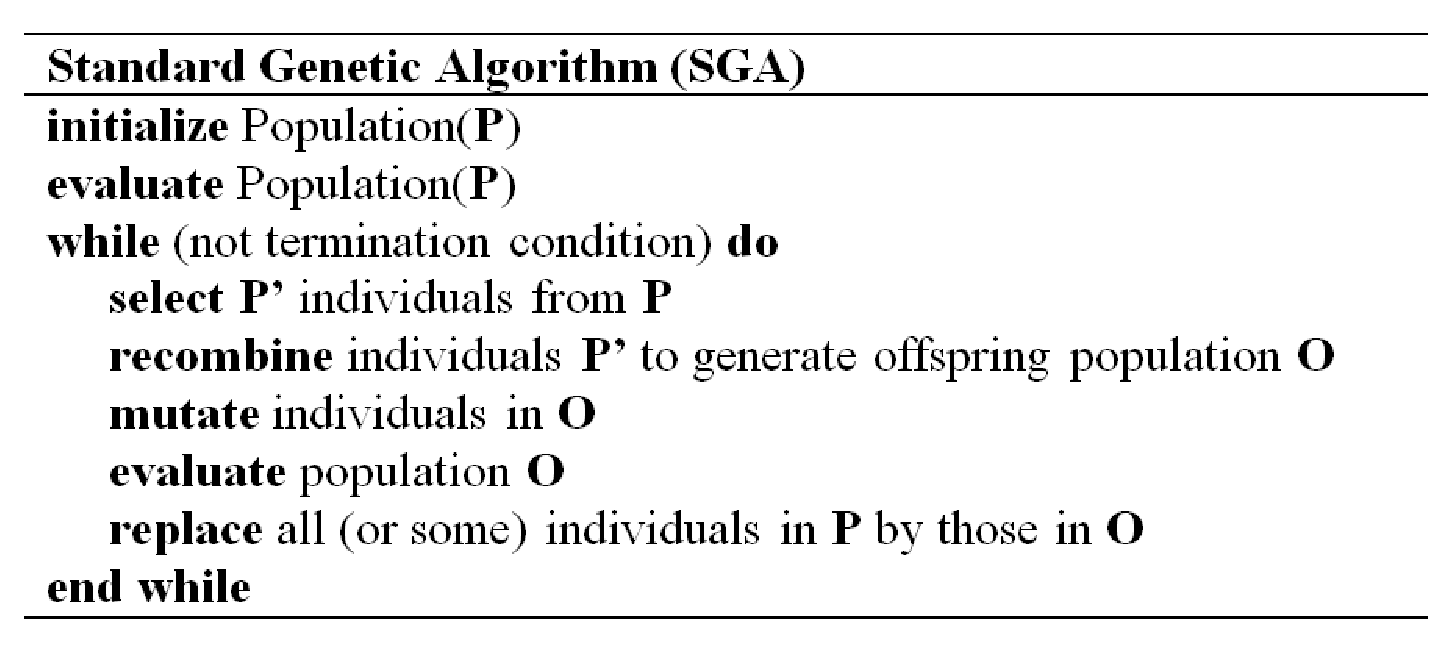
\includegraphics[scale=0.45]{img/GA_pseudocode.eps}
		\caption{Standard GA pseudocode.
		\label{fig:GA_pseudocode}}
	\end{center}
\end{figure}

In the following, the elements comprising the GA implemented to optimize flocking strategies for the Ghost Team are described.

\subsubsection{Initial Population}
\label{par:GA_Initial}

To provide the highest degree of genetic variability to the GA, the
initial population is created as a random set of flocking strategies
defined as: % it always is - JJ

\begin{equation}
	\label{eq:init_dist}
	\forall s \in S, a \in A,  i = 1, \ldots, N, \quad \phi^d_i \sim U(\phi^d_{i-1},\infty)
\end{equation}
\begin{equation}
	\label{eq:init_magn}
	\forall s \in S, a \in A,  i = 1, \ldots, N, \quad \phi^m_i \sim N(0,1/3), \phi^m_i \in [-1,1]
\end{equation}

The elements of $\phi^d$ have a uniform distribution, while the elements of $\phi^m$ have a truncated normal distribution. The parameters of the normal distribution have been set so as to generate most of the magnitudes close to zero.

\subsubsection{Fitness Function}
\label{subsubsec:GA_Fitness}

The definition of the fitness function is one of the most critical
aspects in a GA. The optimization algorithm proposed should generate
Ghost Teams strategies that perform well against any possible
Ms. Pac-Man strategy and, at the same time, are resilient to the
random ghosts direction reverse events (see Section
\ref{sec:mspacman_problem}). To achieve this result, each flocking
strategy is pitted against two different Ms. Pac-Man controllers,
included in the Ms. Pac-Man vs Ghosts competition framework:
\textit{StarterPacMan} (SPM) and \textit{NearestPillPacMan}
(NPPM). The game is simulated 30 times for each Ms. Pac-Man
controller. Thanks to that we can take advantage of the central limit
theorem to compute a relatively precise 95\% confidence interval of
the final score obtained by the Ms. Pac-Man controllers. Let
$\mu_\mathrm{SPM}$, $\sigma_\mathrm{SPM}$, $\mu_\mathrm{NPPM}$,
$\sigma_\mathrm{NPPM}$ be the average score obtained by controller SPM
in the 30 runs, the standard deviation of the SPM's scores, the
average score obtained by controller NPPM in the 30 runs, and the
standard deviation of these scores, respectively. The upper limits of
the confidence intervals for the scores of the two controllers are: % no son muy b�sicos estos dos controladores? �No deber�as usar alguno de los ganadores - JJ 

$$\overline{\mathrm{CI}}_\mathrm{SPM} = \mu_\mathrm{SPM} + Z \cdot \frac{\sigma_\mathrm{SPM}}{\sqrt{30}}$$
$$\overline{\mathrm{CI}}_\mathrm{NPPM} = \mu_\mathrm{NPPM} + Z \cdot \frac{\sigma_\mathrm{NPPM}}{\sqrt{30}}$$

where $Z$ is the 95\% percentile of the standard normal distribution. The upper limits of the confidence intervals represent the maximum score that the Ms. Pac-Man controllers should get 95\% of the times. Our objective is to obtain a Ghost Team controller that minimizes these two values. The fitness function can be now defined as:

$$\mathrm{FITNESS} = \frac{0.7}{\overline{\mathrm{CI}}_\mathrm{SPM}} + \frac{0.3}{\overline{\mathrm{CI}}_\mathrm{NPPM}}$$

% Agh, funci�n agregativa... Hay que justificar esos porcentajes muy
% bien. Yo no pondr�a ninguno, o si acaso poner el ganarle en un 95%
% de los casos al SPM como condici�n. - JJ
The fitness function is basically the weighted average of the confidence intervals' inverses. A bigger weight has been assigned to SPM as it is more complex than NPPM in terms of behavior.

\subsubsection{Selection, Recombination, and Mutation}
\label{subsubsec:GA_Selection_Recombination_Mutation}

After all the strategies of the current generation have been evaluated, it is possible to generate the individuals of the next generation. For each strategy $\Phi$ to be generated, two flocking strategies $\Phi_1$ and $\Phi_2$ are chosen by \textit{roulette-wheel selection}  (i.e., every individual has a probability of being chosen proportional to its fitness). Strategy $\Phi$ is created by random recombination of the parameters of $\Phi_1$ and $\Phi_2$:

$$\forall s \in S, a \in A,  i = 1, \ldots, N, \quad \phi^d_i  = \mathrm{rand}(\phi^d_i \in \Phi_1(s,a), \phi^d_i \in \Phi_2(s,a))$$
$$\forall s \in S, a \in A,  i = 1, \ldots, N, \quad \phi^m_i = \mathrm{rand}(\phi^d_i \in \Phi_1(s,a), \phi^d_i \in \Phi_2(s,a))$$

where \textit{rand} is a function that returns a random value chosen
among its arguments. During the recombination, mutations can occur
with probability $p^\mathrm{mut}$. When a mutation happens, the
current element is re-initialized to a random value, according to
Formulas (\ref{eq:init_dist}) and (\ref{eq:init_magn}). % es un GA
                                % est�ndar. No hay que darle tantas
                                % vueltas, la gente se lo sabe - JJ

The mutation probability $p^\mathrm{mut}$ is determined
dynamically. Initially, its value is set to $p^\mathrm{mut} =
0.00125$. At each iteration $t$, its value changes depending on the
coefficient of variation of the current population fitness, $c_v$: 
% Por qu�? No funciona bien el GA est�ndar? Cualquier experimento de
% este estilo debe justificarse - JJ

$$ p^\mathrm{mut}_t = \left\{
\begin{array}{l l}
	0.00125 & \quad \textrm{if $c_v > 0.6$}\\
	p^\mathrm{mut}_{t-1} & \quad \textrm {if $0.3 < c_v \leq 0.6$}\\
	2 \cdot p^\mathrm{mut}_{t-1} & \quad \textrm {if $0.2 < c_v \leq 0.3$}\\
	4 \cdot p^\mathrm{mut}_{t-1} & \quad \textrm {if $0.1 < c_v \leq 0.2$}\\
	8 \cdot p^\mathrm{mut}_{t-1} & \quad \textrm {if $c_v \leq 0.1$}\\
   \end{array} \right.$$

$c_v$ measures the degree of variability of the population in terms of fitness. When the variability is low, we increment the mutation probability to introduce new chromosomes in the genetic pool of the population. When the variability is too big, the mutation probability is set to a low initial value.

Once the recombination is done and the new Flocking Strategy is created, all its vectors $\phi^d_i$ and $\phi^m_i $ are sorted in ascending order with respect to the values of $\phi^m_i $, to preserve the feasibility of the Flocking Rules.

% No queda claro qu� codificaci�n usas para las estrategias, tama�o
% del cromosoma, esas cosas - JJ
%
%     %%%%%%%%%%   EXPERIMENTS   %%%%%%%%%%
%

\section{Experiments and Results}
\label{sec:experiments}

In the experiments, the GA described in the previous chapter has been
run for 50 generations with a population of 50 candidate %why?
                                %Justificar siempre n�meros m�gicos o
                                %probar diferentes tama�os - JJ
strategies. At each iteration, the next generation was constituted by
49 recombined individuals plus the best solution of the current
generation. 

All the algorithm have been implemented in Java within the framework provided for the Ms Pac-Man vs Ghosts competition. The final program run on a Intel(R) Core(TM) i5-2500K @ 3.3GHz with four cores and 4GB of RAM. Each experiment run on a single core and made use of less than 300MB of memory.

% No comparison with a standard controller? Or a baseline? - JJ

The first experiment regards the comparison of the performance of the Ghost Team controllers obtained with different values of the parameter $N$ (i.e., the number of neighborhoods considered in the Flocking Rules). The best strategy found with a certain number of neighborhoods should be at least as good as those found with a lower number of neighborhoods, as the solution space of the former is bigger and contains the others'. Nevertheless, as the number of neighborhoods increases, the solution space increases substantially, that in turn could affect the actual performance of the GA. In the experiments we use the inverse fitness, $\mathrm{FITNESS}^-1$, as a measure of performance as it is easier to interpret than the fitness function that takes values close to zero. Being the inverse of the fitness value, a lower $\mathrm{FITNESS}^-1$ value corresponds to a better controller, and vice-versa. 

\begin{table} [htbp]
\centering
{\footnotesize
\begin{tabular}{|p{2cm}||c|c|c|c|c|}
\hline & $N = 1$ & $N = 2$ & $N = 3$ & $N = 4$ & $N = 5$ \\
\hline
Best $\mathrm{FITNESS}^-1$ & 1,751.41 & 1,452.54 & 1,484 & 1,489.13 & 1,403.33 \\
\hline
Avg. $\mathrm{FITNESS}^-1$ & 1,870.75 & 1,633.08 & 1,586.84 & 1,545.49 & 1,689.20 \\
\hline
Worst $\mathrm{FITNESS}^-1$ & 1,980.36 & 1,737.86 & 1,712.54 & 1,633.03 & 1,959.05 \\
\hline
Mean \mbox{optimization} time (s) & 1,114 & 1,225 & 1,293 & 1,246 & 1,202 \\
\hline
\end{tabular}}
\caption{Performance of the controllers for the Ghost Team obtained by the GA.
\label{tab:results_GA}}
\end{table}

Table \ref{tab:results_GA} shows the performance of the evolved controllers over three runs of the GA with $N=1,\ldots,5$. Each column is associated to a different number of neighborhoods. The first row displays the inverse fitness of the best individual found. The second rows presents the average controllers fitness, while the third illustrates the fitness value of the worst controller found. Finally, the last row reports the average optimization CPU time over the three runs. By observing the table the following conclusions can be drawn:

\begin{itemize}
	\item The best controller is obtained with $N=5$.
	\item By observing the Avg. $\mathrm{FITNESS}^-1$ row it easy to see that, as the value of $N$ increases, the average performance of the controllers tends to improve as well. The experiments with $N=5$ represent an exception and this could be due to the increased complexity in the search space resulting from the high number of parameters to be optimized by the GA.
	\item For the fitness function considered, two neighborhood areas are sufficient to generate a very efficient controller.
	\item The gap between the best and the worst fitness in each column suggests that the problem presents many local optima in the solution space.
	\item Concerning the optimization time, it seems that it is basically unaffected by changes in the value of $N$. The small difference in the computational time might depend on factors such as memory and CPU usage by other processes.
\end{itemize}

When playing against the best Ghost Team controller obtained by the GA
it is possible to observe complex behaviors. Figure
\ref{fig:GA_Ghost_Behavior} illustrates an example: despite the lack
of coordination between them, the ghosts managed to corral and
surround Ms. Pac-Man that is now entrapped in a corridor. % Enlace a
                                % video (siempre que se pueda mantener
                                % an�nimo) - JJ

\begin{figure}[ht]
	\begin{center}
		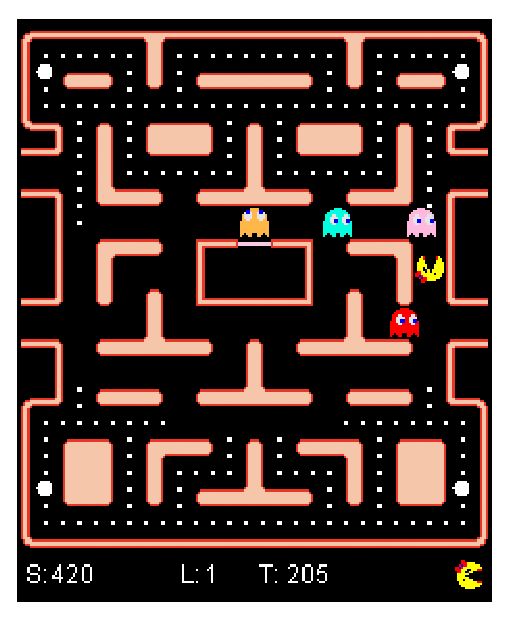
\includegraphics[scale=0.45]{img/ghost_corral.eps}
		\caption{Example of emerging behavior. The ghosts surrounded and entrapped Ms. Pac-Man.
		\label{fig:GA_Ghost_Behavior}}
	\end{center}
\end{figure}

In the next experiment, we compare our controllers with the five Ghost Team controllers included in the competition framework. Their $\mathrm{FITNESS}^-1$ values, computed exactly as per the GA solutions, are the following:

\begin{itemize}
	\item \textit{AggressiveGhosts} : 4,645.79;
	\item \textit{Legacy} : 4,577.61;
	\item \textit{Legacy2TheReckoning} : 3,631.94;
	\item \textit{RandomGhosts} : 12,205.60;
	\item \textit{StarterGhosts} : 3,785.49;
\end{itemize}

According to these results, the best controller is
\textit{Legacy2TheReckoning}, followed by
\textit{StarterGhosts}. Nevertheless, their $\mathrm{FITNESS}^-1$
value is more than three times bigger than that of the best evolved
flocking strategy. These results support the claim that flocking
strategies are a viable option for the definition of intelligent
controllers. % Pero no por qu� no hab�is usado esos controladores en
             % el entrenamiento. �Por qu� no pones la puntuaci�n? - JJ 

% Por otro lado, habr�a que describir el juego de los controladores
% que han evolucionado. - JJ

%
%     %%%%%%%%%%   CONCLUSIONS  %%%%%%%%%%
%

\section{Conclusions and Future Work}
\label{sec:conclusions}

In this paper, a new controller for the Ghost Team based on flocking
strategies is proposed. A GA is presented to design optimized
strategies offline. The methodology has been empirically tested. The
results show that flocking strategies, despite the reduced
computational cost, % Reducido �con respecto a qu�? no has probado nada de esto. �Cu�l es el coste
                    % computacional de otros? - JJ
 model complex behaviors and produce effective and challenging agents. This work is just scratching the surface and there is still a lot to be investigated. Some possible future lines of research are highlighted in the following.

The fitness function can be easily extended by including more Ms. Pac-Man controller. This should result in a Ghost Team controller that performs better against a wider range of opponents. By considering in the GA fitness function the best Ms. Pac-Man controllers that took part to the competitions, it would be possible to generate Ghost Team controllers that are capable of tackling the best known Ms. Pac-Man strategies.

Moreover, it would be interesting to compare the controllers obtained by applying the presented methodology with the best Ghost Team controllers that took part to the Ms. Pac-Man vs Ghosts competition. This would allow us to really understand the limits of Flocking Strategies.

The GAs as a means to optimize Flocking Strategies have proven to be satisfactory. Nevertheless, the recombination step causes abrupt changes in the solutions' parameters and might generate individuals that are very different from the initial ones. It would be interesting to investigate the effectiveness of optimization methods that allows for small changes in the solutions parameters. Particle Swarm Optimization (PSO) algorithms  might be a sensible choice. In fact, on top of making few or no assumptions about the problem, PSO algorithm are particularly effective with problems that are noisy and present many multiple optima, such as this one.

We hope that this work will be a useful source of ideas for future research on bio-inspired algorithms in games and will contribute further in the development and solution of more complex problems.

%
%     %%%%%%%%%%   ACKNOWLEDGMENTS  %%%%%%%%%%
%

%\section*{Acknowledgments}
%This work has been supported in part by EVORQ, CANUBE, etc, and the TIN2011-28627-C04-02 project, awarded by the Spanish Ministry of Science and Innovation. Liberatore's research was financed by the Government of Spain (TIN2012-32482). Also, Liberatore would like to thanks the GeNeura research group at University of Granada for their kind hospitality. All the supports are gratefully acknowledged.

\bibliographystyle{splncs}

\bibliography{flocking_pacman}

\end{document}
